% SPDX-License-Identifier: CC-BY-4.0
% Copyright (c) 2026 Alexander S. Donahue
% SecMesh-PQSI v3.0.0 -- 3-Page NIST-Aligned Cyber & Quantum Technical Executive Brief
\documentclass[10pt,letterpaper]{article}

\usepackage[T1]{fontenc}
\usepackage[utf8]{inputenc}
\usepackage{lmodern}
\usepackage{microtype}
\usepackage[margin=0.45in,top=0.56in,bottom=0.46in,headheight=12pt,headsep=8pt,footskip=14pt]{geometry}
\usepackage{amsmath,amssymb}
\usepackage{xcolor}
\usepackage{booktabs}
\usepackage{tabularx}
\usepackage{ragged2e}
\usepackage{enumitem}
\usepackage[most]{tcolorbox}
\usepackage{tikz}
\usetikzlibrary{arrows.meta,positioning,calc}
\usepackage{fancyhdr}
\usepackage{titlesec}
\usepackage[hidelinks,
  pdftitle={SecMesh-PQSI v3.0.0: NIST-Aligned Post-Quantum and Information-Theoretic Cyber Defense},
  pdfauthor={Alexander S. Donahue},
  pdfsubject={Post-Quantum Cryptography, NIST FIPS 203/204/205, Quantum Information Theory, Lean 4 Formal Verification}
]{hyperref}

% Palette -- NIST Navy + Quantum Teal + Slate + Emerald + Amber
\definecolor{nistnavy}{HTML}{0F2A47}
\definecolor{qteal}{HTML}{0E7490}
\definecolor{emgreen}{HTML}{047857}
\definecolor{warnamber}{HTML}{B45309}
\definecolor{softbg}{HTML}{F4F7FA}
\definecolor{tealbg}{HTML}{EFF9FB}
\definecolor{amberbg}{HTML}{FFFBEB}
\definecolor{slatext}{HTML}{334155}
\definecolor{rulecol}{HTML}{CBD5E1}

\newcolumntype{Y}{>{\RaggedRight\arraybackslash}X}
\newcolumntype{L}[1]{>{\RaggedRight\arraybackslash}p{#1}}
\newcommand{\code}[1]{\texttt{\fontsize{7.8pt}{9.2pt}\selectfont #1}}

% Crisp, compact section styling
\titleformat{\section}{\fontsize{10.5pt}{12pt}\selectfont\bfseries\color{nistnavy}}{}{0pt}{}[\vspace{-3pt}\textcolor{qteal}{\titlerule[0.75pt]}]
\titlespacing*{\section}{0pt}{6.5pt}{3.5pt}

% Header & Footer
\pagestyle{fancy}
\fancyhf{}
\renewcommand{\headrulewidth}{0.4pt}
\renewcommand{\headrule}{\hbox to\headwidth{\color{rulecol}\leaders\hrule height \headrulewidth\hfill}}
\lhead{\scriptsize\color{slatext}\textbf{SecMesh-PQSI v3.0.0} \;|\; NIST Cyber \& Quantum Technical Executive Brief}
\rhead{\scriptsize\color{slatext}Alexander S.\ Donahue \;(\texttt{ORCID 0009-0006-8168-9648})}
\lfoot{\scriptsize\color{slatext}Repo: \href{https://github.com/0thernes/secmesh-pqsi}{\texttt{github.com/0thernes/secmesh-pqsi}} \;\textbullet\; Console: \href{https://0thernes.github.io/secmesh-pqsi/}{\texttt{0thernes.github.io/secmesh-pqsi}} \;\textbullet\; Archive: \texttt{0TH-2026-011}}
\rfoot{\scriptsize\color{slatext}\textbf{Page \thepage\ of 3}}
\setlength{\parindent}{0pt}
\setlength{\parskip}{2.4pt}

\tcbset{
  briefbox/.style={
    colback=softbg, colframe=nistnavy, boxrule=0.6pt, arc=2pt,
    left=6pt, right=6pt, top=4.5pt, bottom=4pt, fonttitle=\bfseries\footnotesize\color{white},
    fontupper=\fontsize{8.2pt}{10.0pt}\selectfont,
    colbacktitle=nistnavy, attach boxed title to top left={yshift=-2mm, xshift=3mm},
    boxed title style={arc=1.5pt, boxrule=0pt, top=1.3pt, bottom=1.3pt, left=5pt, right=5pt},
    enhanced
  },
  tealbox/.style={
    colback=tealbg, colframe=qteal, boxrule=0.6pt, arc=2pt,
    left=6pt, right=6pt, top=4pt, bottom=3.5pt, fonttitle=\bfseries\scriptsize\color{white},
    fontupper=\fontsize{7.9pt}{9.6pt}\selectfont,
    colbacktitle=qteal, attach boxed title to top left={yshift=-1.8mm, xshift=3mm},
    boxed title style={arc=1.5pt, boxrule=0pt, top=1.2pt, bottom=1.2pt, left=5pt, right=5pt},
    enhanced
  },
  amberbox/.style={
    colback=amberbg, colframe=warnamber, boxrule=0.6pt, arc=2pt,
    left=6pt, right=6pt, top=4pt, bottom=3.5pt, fonttitle=\bfseries\scriptsize\color{white},
    fontupper=\fontsize{7.9pt}{9.6pt}\selectfont,
    colbacktitle=warnamber, attach boxed title to top left={yshift=-1.8mm, xshift=3mm},
    boxed title style={arc=1.5pt, boxrule=0pt, top=1.2pt, bottom=1.2pt, left=5pt, right=5pt},
    enhanced
  }
}

\begin{document}
\fontsize{8.4pt}{10.2pt}\selectfont
\thispagestyle{empty}

% ============================ PAGE 1 ============================
\vspace*{-0.16in}
\begin{tcolorbox}[colback=nistnavy, colframe=nistnavy, arc=3pt, left=8pt, right=8pt, top=6.5pt, bottom=6.5pt, boxrule=0pt]
  {\fontsize{7.2pt}{8.5pt}\selectfont\color{cyan!30}\textbf{NIST-ALIGNED CYBERSECURITY \& QUANTUM INFORMATION TECHNICAL BRIEF}\hfill\textbf{RELEASE v3.0.0 \;|\; NOV 2026}}\\[2.5pt]
  {\fontsize{13.8pt}{15.8pt}\selectfont\bfseries\color{white}SecMesh-PQSI: Post-Quantum and Information-Theoretic Cyber Defense}\\[2pt]
  {\fontsize{7.8pt}{9.4pt}\selectfont\color{white!90}Scientific \& Engineering Guide to NIST FIPS~203/204/205 Hybrid Mesh Security, Six-Kernel Formal Proofs, and Quantum Geometry}\\[3pt]
  {\fontsize{7.0pt}{8.2pt}\selectfont\color{cyan!20}\textbf{Author:} Alexander S.\ Donahue (Spokane, WA \;\textbullet\; \href{https://orcid.org/0009-0006-8168-9648}{\color{cyan!20}\texttt{ORCID 0009-0006-8168-9648}} \;\textbullet\; \texttt{0\_0@0thernes.art})\hfill\textbf{Licenses:} Apache-2.0 / MIT / CC-BY-4.0}
\end{tcolorbox}
\vspace{1pt}

\begin{tcolorbox}[briefbox, title={Executive Summary --- What We Built and Why It Matters}]
Today's internet encryption (RSA, Diffie--Hellman, and elliptic curves such as X25519/Ed25519) faces two distinct horizons. First, \textbf{Store-Now, Decrypt-Later (SNDL)} adversaries can harvest encrypted traffic today and break it once fault-tolerant quantum computers run \textbf{Shor's algorithm}. Second, a hypothetical \textbf{Post-Super-Intelligence (PSI)} adversary could someday discover unforeseen polynomial-time math breakthroughs against structured post-quantum assumptions like lattices.
\textbf{SecMesh-PQSI v3.0.0} is a clean-room cryptographic defense engine rebuilt atop Tsotchke's audited 27-repository open-source stack (\code{moonlab}, \code{quantum\_geometric\_tensor}, \code{libirrep}, \code{spin\_based\_neural\_network}, \code{eshkol}, \code{rosette-wire}, \code{pq-consensus-bandwidth}). It fuses \textbf{NIST FIPS~203/204/205} post-quantum cryptography with an optional \textbf{information-theoretic (math-only) layer}, backed by \textbf{28 machine-checked zero-Mathlib Lean~4.35.0 theorems} verified independently by \textbf{all six distinct Lean proof kernels}, bit-exact C11 $\leftrightarrow$ OpenSSL~3.5.5 FIPS~203 interoperability, and 12 documented security hardening cycles.
\end{tcolorbox}

\section{1. Can Shor, Grover, or Brute Force Break It? (The Threat Matrix)}
A practical way to judge any quantum-era security tool is to ask exactly which attacker class breaks which layer. Table~\ref{tab:threats} separates what is stopped by \textbf{NIST post-quantum algorithms alone} from what requires \textbf{independent physical or pre-shared randomness}---a boundary enforced by Claude Shannon's 1949 secrecy theorem rather than engineering preference.

\begin{table}[h!]
\centering
\vspace{-4pt}
\fontsize{7.9pt}{9.6pt}\selectfont
\renewcommand{\arraystretch}{1.15}
\begin{tabularx}{\linewidth}{@{}L{2.75cm} L{2.45cm} Y L{3.35cm}@{}}
\toprule
\textbf{Attacker Class} & \textbf{Attack Vector} & \textbf{SecMesh-PQSI Defense Layer \& NIST Anchor} & \textbf{Security Status} \\
\midrule
\textbf{Classical Network Attacker} & MITM, replay, DoS, forged tags, key-harvesting & Hybrid \code{X25519+ML-KEM-768}, \code{AES-256-GCM} (strict 128-bit tag, SP~800-38D), RFC-6479 sliding replay window, HTTP~405/CSP/Slowloris Guardian~v2. & \textcolor{emgreen}{\textbf{BLOCKED}} ($2^{256}$ symmetric; $2^{128}$ auth tag). \\
\textbf{Fault-Tolerant Quantum Computer} & \textbf{Shor's algorithm} (breaks RSA / ECC) & \textbf{NIST FIPS~203} (\code{ML-KEM-768}) + \textbf{FIPS~204} (\code{ML-DSA-65}) + optional \textbf{FIPS~205} (\code{SLH-DSA-128s} hash-based) fused via XOR dual-survivability (\textbf{T2b}). & \textcolor{emgreen}{\textbf{BLOCKED}} (Shor does not apply to lattices or hashes). \\
\textbf{Quantum Brute Force} & \textbf{Grover's algorithm} ($\sqrt{N}$ search speedup) & Full 256-bit keys across \code{AES-256-GCM} (FIPS~197) and \code{SHAKE-256} (FIPS~202); Grover cuts $2^{256}$ only to $2^{128}$ sequential quantum oracle queries. & \textcolor{emgreen}{\textbf{BLOCKED}} ($2^{128}$ quantum steps physically infeasible). \\
\textbf{Post-Super-Intelligence (Infinite Compute)} & Arbitrary math breakthroughs against lattices/AES & \textbf{Optional PSI Lane} (\code{SECMESH\_IT\_PAD\_FILE}): One-Time Pad XOR (\textbf{T2a}) + one-time $\mathbb{F}_{2^{128}}$ Carter--Wegman MAC (\textbf{T2d}) + Byzantine Shamir split (\textbf{T3a--T3b}). & \textcolor{emgreen}{\textbf{BLOCKED with pad}} (PQ-only mode reduces to FIPS~203/205). \\
\bottomrule
\end{tabularx}
\vspace{-4pt}
\caption{\scriptsize Attacker capability matrix distinguishing computational post-quantum guarantees from unconditional information-theoretic (PSI) guarantees.}
\label{tab:threats}
\vspace{-6pt}
\end{table}

\section{2. Layered Defense Architecture (How a Packet Stays Safe)}
Instead of betting everything on a single mathematical assumption, \code{SecMesh-PQSI} uses a \textbf{dual-survivability combiner} (Theorem~\textbf{T2b}): every session key combines independent secrets from classical, lattice, hash-based, and (optionally) physical/pre-shared random sources. An attacker must break \emph{every active layer simultaneously}.

\begin{figure}[h!]
\centering
\vspace{-3pt}
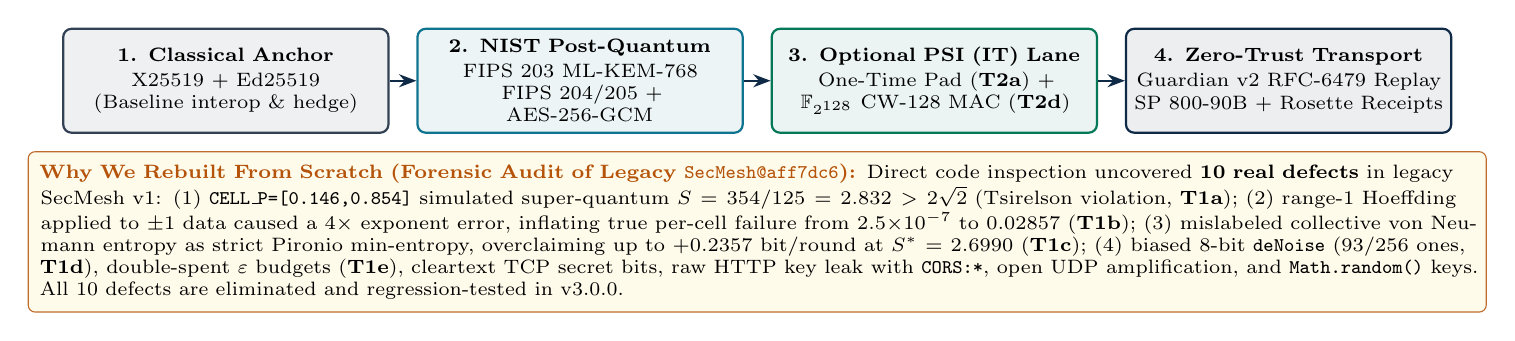
\begin{tikzpicture}[
  font=\scriptsize,
  layer/.style={draw=#1, fill=#1!8, rounded corners=3pt, line width=0.8pt,
                minimum height=1.32cm, text width=3.92cm, align=center, inner sep=3pt},
  arr/.style={-{Stealth[length=2.2mm]}, line width=0.85pt, draw=nistnavy}
]
  \node[layer=slatext] (L1) {\textbf{1. Classical Anchor}\\[1pt]X25519 + Ed25519\\(Baseline interop \& hedge)};
  \node[layer=qteal, right=0.34cm of L1] (L2) {\textbf{2. NIST Post-Quantum}\\[1pt]FIPS~203 ML-KEM-768\\FIPS~204/205 + AES-256-GCM};
  \node[layer=emgreen, right=0.34cm of L2] (L3) {\textbf{3. Optional PSI (IT) Lane}\\[1pt]One-Time Pad (\textbf{T2a}) +\\$\mathbb{F}_{2^{128}}$ CW-128 MAC (\textbf{T2d})};
  \node[layer=nistnavy, right=0.34cm of L3] (L4) {\textbf{4. Zero-Trust Transport}\\[1pt]Guardian~v2 RFC-6479 Replay\\SP~800-90B + Rosette Receipts};

  \draw[arr] (L1) -- (L2);
  \draw[arr] (L2) -- (L3);
  \draw[arr] (L3) -- (L4);

  \coordinate (midBot) at ($(L1.south west)!0.5!(L4.south east)$);
  \node[below=0.22cm of midBot, anchor=north, draw=warnamber!85, fill=amberbg,
        rounded corners=2.5pt, text width=18.2cm, align=left, inner sep=4.5pt, font=\scriptsize] (forensic) {
    \textbf{\textcolor{warnamber}{Why We Rebuilt From Scratch (Forensic Audit of Legacy \texttt{SecMesh@aff7dc6}):}}
    Direct code inspection uncovered \textbf{10 real defects} in legacy SecMesh~v1: (1)~\texttt{CELL\_P=[0.146,0.854]} simulated super-quantum $S=354/125=2.832 > 2\sqrt{2}$ (Tsirelson violation, \textbf{T1a}); (2)~range-1 Hoeffding applied to $\pm 1$ data caused a $4\times$ exponent error, inflating true per-cell failure from $2.5{\times}10^{-7}$ to $0.02857$ (\textbf{T1b}); (3)~mislabeled collective von Neumann entropy as strict Pironio min-entropy, overclaiming up to $+0.2357$ bit/round at $S^*=2.6990$ (\textbf{T1c}); (4)~biased 8-bit \texttt{deNoise} ($93/256$ ones, \textbf{T1d}), double-spent $\varepsilon$ budgets (\textbf{T1e}), cleartext TCP secret bits, raw HTTP key leak with \texttt{CORS:*}, open UDP amplification, and \texttt{Math.random()} keys. All 10 defects are eliminated and regression-tested in v3.0.0.
  };
\end{tikzpicture}
\vspace{-6pt}
\caption{\scriptsize End-to-end SecMesh-PQSI defense pipeline: classical baseline, NIST FIPS~203/204/205 post-quantum cryptography, optional unconditional information-theoretic masking, and Zero-Trust hardened transport with verifiable Rosette-Wire audit receipts.}
\label{fig:arch}
\end{figure}

% ============================ PAGE 2 ============================
\newpage
\section{3. The Science Behind the Code: 28 Machine-Checked Theorems Across 6 Kernels}
In cryptography and quantum information, subtle algebra or boundary errors routinely slip past human reading---as our forensic audit of legacy SecMesh demonstrated. To eliminate hidden logic gaps, we formalized \textbf{all 28 core mathematical claims} in \textbf{Lean~4.35.0} with \textbf{zero Mathlib dependencies} (15 source files, 5,133 lines, 0 warnings, 0 proof \code{sorry}s, 0 \code{native\_decide}).

\textbf{What ``Six-Kernel Verification'' Means in Plain English:} Think of a Lean proof as source code whose compiler checks mathematical logic instead of syntax. Rather than trusting a single proof checker, our continuous integration pipeline replays all 28 theorems, concrete non-vacuity witnesses (\code{SimpleField (Fin 5)} and finite graphs confirming no hypothesis is trivially empty), and \textbf{5 zero-axiom adversarial boundary counterexamples} (\textbf{63 audited declarations} total) through \textbf{six independent kernel implementations} via \code{lake comparator --paranoid}: \code{Lean paranoid}, \code{lean4lean}, \code{nanoda}, \code{con-leche --verified} (3,713/3,764 decls), \code{con-ron --verified}, and \code{Lean default}. Every theorem depends strictly on Lean's standard foundational axioms \code{[propext, Classical.choice, Quot.sound]}---and our CI runs a live negative test proving the kernel rejects a deliberately false FIPS~203 \code{Compress\_1} theorem.

\begin{table}[h!]
\centering
\vspace{-4pt}
\fontsize{7.4pt}{8.9pt}\selectfont
\renewcommand{\arraystretch}{1.08}
\begin{tabularx}{\linewidth}{@{}L{1.45cm} L{2.95cm} L{5.10cm} Y@{}}
\toprule
\textbf{Family} & \textbf{Plain-English Meaning} & \textbf{Exact Proved Law (Lean 4.35)} & \textbf{Engineering \& Research Impact} \\
\midrule
\textbf{T1a--T1e} & Forensic DI-QKD Finite-Key Audit & $354^2{-}8{\cdot}125^2 = 316 > 0$; $u^2{+}v^2=1$ ($\Delta_{\max}=+0.235703$ at $S^*=2.698960$); 5-lane $\sum\varepsilon_i \le \varepsilon_{\mathrm{tot}}$. & Fixes all 10 legacy SecMesh bugs; replaces ad-hoc bounds with exact Bernoulli Chernoff--KL QBER inversion. \\
\textbf{T2a--T2d} & Unconditional PSI Cryptographic Triad & OTP bijection; $k$-factor XOR combiner; Toeplitz 2-universality; integer LHL; poly MAC $\le d/|\mathbb{F}|$. & Guarantees confidentiality \& authenticity against infinite compute whenever a fresh independent pad is supplied. \\
\textbf{T3a--T3c} & Byzantine Secret Sharing \& PIR & Shamir $(t,n)$ secrecy; Singleton bound $n \ge t{+}2b$ (tight at $n{=}t{+}2b{-}1$); \code{CS-053} gap $T^2 > 0$. & Eliminates single-node compromise even with $b$ lying nodes; quantifies exact gap in Mega Atlas \code{CS-053}. \\
\textbf{T4a--T4e} & Quantum Geometry, Chern Law \& qLDPC & $\det(g){-}\tfrac{1}{4}\Omega^2 = \tfrac{1}{4}\mathcal{C}^2\sin^2(\tfrac{\theta}{2})$; $c_{\mathrm{eff}}^2{+}\mathcal{C}^2=1$; GHZ QFI $N^2\tau_N$; BB144 5,184 CSS checks. & Links Tsotchke's \code{QGTL} \& \code{libirrep} directly to Bell entanglement \& certifies Bravyi's $[[144,12,12]]$ qLDPC code. \\
\textbf{T5a--T5d} & NIST FIPS~203 Lattice Math \& Bandwidth & $q{=}3329$ prime, $\zeta{=}17$ 256th root; zero-overflow Montgomery; \code{Compress\_1} $|e|\le 831$ (tight $+832$); $K_N$ ceiling. & Guarantees exact FIPS~203 polynomial arithmetic without silent overflow; proves IT-MAC adds $<1.75\%$ wire overhead. \\
\textbf{T6a--T6b} & Cyber-Contagion Barrier \& Subliminals & Laplacian PSD; Ising cut bijection; Cheeger work $W_{\min}(k)\ge 2k(J_{\min}\phi_0{+}h_{\min})$; XOR nonce closure. & Translates expander graph connectivity into a provable work barrier against malware spread \& kleptographic leaks. \\
\textbf{T7a--T7c} & Quantum Monogamy, No-Go \& Microcrypt & $S_{AB}^2{+}S_{AE}^2\le 8$; $\mathrm{TV}{+}\mathrm{Overlap}=1$; $1{-}B\le\mathrm{TV}$, $\mathrm{TV}^2{+}B^2\le 1$, $D_{\mathrm{tr}}^2{+}F=1$ (\code{CS-031}/\code{QC-022}). & Traps quantum eavesdroppers below classical bound; proves why hybrid PQ+PSI is mathematically required; bounds EFI pairs. \\
\bottomrule
\end{tabularx}
\vspace{-4pt}
\caption{\scriptsize Summary of all 28 zero-Mathlib Lean 4.35.0 theorems across 7 families, verified across 6 independent kernels and cross-checked to 60-digit precision in Python.}
\label{tab:theorems}
\vspace{-6pt}
\end{table}

\section{4. Two Headline Scientific Unifications (Explained Intuitively)}
Beyond verifying standard cryptography, our formalization establishes two structural unifications connecting Tsotchke's quantum-geometry libraries to NIST post-quantum architecture and frontier open conjectures from the \emph{Unsolved Problems Mega Atlas}:

\begin{tcolorbox}[tealbox, title={Unification A --- The Topological Chern--Concurrence--Entropy Conservation Law (Theorem T4d)}]
Consider a two-qubit link parameterized by entanglement angle $\alpha$ (Wootters concurrence $\mathcal{C} = \sin 2\alpha \in [0,1]$) and local Bloch-sphere rotations $(\theta,\phi)$ on Alice's qubit. Computing the Quantum Geometric Tensor (QGT) via Tsotchke's \code{QGTL} yields both the Fubini--Study metric $g$ and the Berry curvature $\Omega_{\theta\phi}$, whose integrated effective local Chern monopole is $c_{\mathrm{eff}} = \cos 2\alpha$. We prove the exact conservation law:
{\setlength{\abovedisplayskip}{3pt}\setlength{\belowdisplayskip}{3pt}
\[
  c_{\mathrm{eff}}^2 + \mathcal{C}^2 = 1
  \qquad\Longleftrightarrow\qquad
  c_{\mathrm{eff}}^2 + \left(\frac{S_{\max}}{2}\right)^{\!2} = 2
  \qquad\Longrightarrow\qquad
  H_{\min}^{\mathrm{DI}}(S_{\max}) = 1 - \log_2\!\bigl(1 + |c_{\mathrm{eff}}|\bigr).
\]}
\textbf{Intuition for engineers:} A quantum link splits a fixed geometric budget of $1$ between \emph{local topological curvature} ($c_{\mathrm{eff}}^2$) and \emph{non-local entanglement} ($\mathcal{C}^2$). For an unentangled state ($\mathcal{C}=0$), local curvature is maximal ($|c_{\mathrm{eff}}|=1$) and certified randomness is $0$. As entanglement approaches a singlet ($\mathcal{C}\to 1$), the local Berry monopole drains completely ($c_{\mathrm{eff}}\to 0$), unlocking $1$ full bit of Pironio device-independent min-entropy per round (verified to $10^{-59}$ in 60-digit arithmetic).
\end{tcolorbox}
\vspace{1pt}

\begin{tcolorbox}[tealbox, title={Unification B --- Why Hybrid PQ+PSI Is Mathematically Inevitable (Theorems T7b \& T7c)}]
Can a single protocol achieve \emph{unconditional} security for every cryptographic task without computational hardness? Theorems~\textbf{T7b} and~\textbf{T7c} formalize the exact quantitative barrier. For any two candidate distributions or quantum states with total variation / trace distance $\mathrm{TV}$ ($D_{\mathrm{tr}}$), classical overlap $\mathrm{Overlap}$, and Bhattacharyya fidelity $B$ ($\sqrt{F}$):
{\setlength{\abovedisplayskip}{3pt}\setlength{\belowdisplayskip}{3pt}
\[
  \mathrm{TV} + \mathrm{Overlap} = 1 \quad(\text{\textbf{T7b}}),
  \qquad
  1 - B \le \mathrm{TV}, \qquad \mathrm{TV}^2 + B^2 \le 1, \qquad D_{\mathrm{tr}}^2 + F = 1 \quad(\text{\textbf{T7c}}).
\]}
\textbf{Intuition for engineers:} Strong hiding forces $\mathrm{TV} \to 0$, which forces fidelity $F \to 1$---allowing an unbounded quantum cheater (Mayers--Lo--Chau) to pivot between openings. Conversely, Quantum Microcrypt's \emph{EFI pairs} (\textbf{Mega Atlas \code{CS-031} \& \code{QC-022}}, quantum crypto weaker than one-way functions) require statistically far states ($\mathrm{TV}\ge\delta$), which our theorem proves forces $B^2 + \delta^2 \le 1$ (saturated tightly by our 0-axiom $(3,4,5)$ Pythagorean witness). \textbf{Architectural takeaway:} Unconditional encryption (OTP) and authentication (CW-128) require pre-shared/physical entropy, while scalable key establishment and signatures require computational hardness (NIST FIPS~203/204/205). Fusing both in a dual-survivability hybrid achieves the exact best of both worlds.
\end{tcolorbox}

% ============================ PAGE 3 ============================
\newpage
\section{5. NIST Cyber Framework Mapping, Implementation \& Hardening Results}
To bridge formal mathematics into deployable software engineering, Table~\ref{tab:nist} maps \code{SecMesh-PQSI v3.0.0} directly onto the \textbf{NIST Cybersecurity Framework (CSF~2.0)}, \textbf{NIST SP~800-207 (Zero Trust)}, and \textbf{NIST Post-Quantum Standards (IR~8547 / FIPS~203--205)}.

\begin{table}[h!]
\centering
\vspace{-4pt}
\fontsize{7.4pt}{8.9pt}\selectfont
\renewcommand{\arraystretch}{1.08}
\begin{tabularx}{\linewidth}{@{}L{2.45cm} L{2.75cm} Y L{4.00cm}@{}}
\toprule
\textbf{NIST CSF 2.0 / Standard} & \textbf{Control Objective} & \textbf{SecMesh-PQSI v3.0.0 Implementation} & \textbf{Verified Hardening Proof (12 Cycles)} \\
\midrule
\textbf{Protect} (FIPS~203, 204, 205; IR~8547) & Quantum-resistant key exchange \& signatures & Vendored MIT C11 \code{moonlab} ML-KEM-768 + Node~25 OpenSSL~3.5.5 hybrid (\code{X25519+ML-KEM-768+ML-DSA-65/SLH-DSA-128s}). & Bit-exact C11 $\leftrightarrow$ OpenSSL~3.5.5 KAT \& FO tamper rejection; \code{6,685 B} std / \code{14,989 B} hedged. \\
\textbf{Protect} (FIPS~197, 202; SP~800-38D) & Authenticated encryption \& domain separation & \code{AES-256-GCM} + \code{SHAKE-256} KDF + canonical \code{u32be}-framed $\mathbb{F}_{2^{128}}$ Carter--Wegman record MAC + optional OTP pad. & Fixed \textbf{CWE-347} tag truncation (\code{authTagLength:16}), strict key/IV checks, \code{finally} secret zeroization. \\
\textbf{Protect / Zero Trust} (SP~800-207) & Replay, DoS \& endpoint control plane & Hardened Guardian~v2: RFC-6479 4,096-seq replay window, 4,096-IP cap, \code{GET/HEAD}-only HTTP~405, Slowloris timeouts, CSP. & Zero UDP echo amplification, loopback-only status, zero raw key exposure, 64~KiB line cap. \\
\textbf{Detect} (SP~800-90B) & Continuous entropy health \& verification & OS CSPRNG (\code{BCryptGenRandom}/\code{getrandom} + \code{EINTR} retry) + SP~800-90B RCT/APT gate + 5 live Eshkol v1.3.6 AD modules. & Parse/eval depth DoS caps (\code{256}), live Eshkol gradients verified $<10^{-12}$, schema-bound Rosette receipts. \\
\textbf{Respond \& Recover} (CSF~2.0) & Contagion containment \& fault tolerance & Expander health-field mesh defense (\textbf{T6a}) + Byzantine Shamir $(t,n)$ secret recovery (\textbf{T3a--T3b}) over $\mathbb{F}_{p}$. & \code{\_\_int128} Ising overflow guard, duplicate-\code{x} forgery block, DFS cap, C stack secret zeroization. \\
\bottomrule
\end{tabularx}
\vspace{-4pt}
\caption{\scriptsize Engineering alignment of SecMesh-PQSI v3.0.0 controls with NIST CSF~2.0, SP~800-207 Zero Trust, SP~800-90B, and FIPS~197/202/203/204/205.}
\label{tab:nist}
\vspace{-6pt}
\end{table}

\section{6. End-to-End Verification Matrix \& Pre-Registered Empirical Benchmark}
Every layer is backed by automated, deterministic verification executed on both Windows~11 (GCC~16.1.0, Node~25.8.2 / OpenSSL~3.5.5, Lean~4.35.0, Python~3.12.10) and Ubuntu Linux CI with Sigstore SLSA build provenance:
{\fontsize{8.0pt}{9.6pt}\selectfont
\begin{itemize}[leftmargin=1.25em,itemsep=1.0pt,topsep=1.0pt,parsep=0pt]
  \item \textbf{Native C11 Core (\code{native/}):} \textbf{69/69 tests passed} under \code{-std=c11 -Wall -Wextra -Werror} (0 warnings) + AddressSanitizer/UBSan + \textbf{500/500 standalone fuzz inputs}; strict CLI parsing (\code{parse\_strict\_double/u64}) rejecting \code{NaN}/garbage tokens.
  \item \textbf{Node.js~25 Interop \& Live Eshkol AD (\code{node/}, \code{eshkol/}):} \textbf{34/34 tests passed}, proving bit-exact C11 $\leftrightarrow$ OpenSSL~3.5.5 FIPS~203 ML-KEM-768 encapsulation/decapsulation, live 25,007~B lattice-hedged handshake RTT, deterministic seeded Toeplitz extraction, and live forward-mode dual-number automatic differentiation across all \textbf{5 Eshkol \code{.esk} modules} (\textbf{T1}--\textbf{T7}).
  \item \textbf{Python Exact Suite, Citations \& Standards Compliance:} \textbf{15/15 pytest passed}, 0 \code{ruff}/0 \code{mypy} errors, \textbf{44/44 live HTTP-200 citations} (33/33 Crossref-checked non-retracted DOIs + 1 DataCite/LIPIcs DOI), \textbf{65/65} LF-idempotent \code{MANIFEST.sha256}, and \textbf{100.0\% (76/76 PASS, 0 warnings)} on Build Standard v1.2.0.
  \item \textbf{Pre-Registered 30-Seed Mesh Contagion Simulation (\code{seeds 20260001..20260030}, 60 nodes, 400 steps):} Comparing undefended Control vs.\ Hardened Treatment (6 defenders, firewall $0.7$) yields \textbf{30/30 strict wins} (rank-biserial $r_{\mathrm{rb}}=1.000$, Holm--Bonferroni $p_{\mathrm{Holm}} = 3.73\times 10^{-9}$): mean admitted intrusions drop from \textbf{60.000} to \textbf{0.033} (nonparametric 10,000-resample bootstrap 95\% CI \code{[59.900, 60.000]}) and peak mesh stress drops from \textbf{1.0425} to \textbf{0.4431} (bootstrap 95\% CI \code{[0.5794, 0.6198]}).
  \item \textbf{Bandwidth Ceilings ($K_N$ All-to-All @ 100~Mbps):} Standard PQ+PSI-MAC (\code{6,685 B} one-way) supports up to \textbf{1,870 peers} per second (only $+112\text{ B} = 1.71\%$ overhead over plain ML-KEM/ML-DSA); Lattice-Hedged SLH-DSA (\code{14,989 B} one-way) supports \textbf{834 peers}.
\end{itemize}}
\vspace{1pt}

\begin{tcolorbox}[amberbox, title={Honest Scientific \& Operational Boundaries (Zero-Hype Disclosure)}]
To uphold Tier-1 scientific integrity, four strict boundaries apply:
\textbf{(1)~Software E91 is a simulator, not laser QKD:} Classical TCP packets cannot close physical Bell detection/locality loopholes; hardware QRNG or physical optical QKD is required for live physical randomness.
\textbf{(2)~PSI unbreakability requires real pad hygiene:} Without an independent, never-reused pad (\code{SECMESH\_IT\_PAD\_FILE}), security reduces to NIST FIPS~203/204/205 computational hardness---still immune to Shor and Grover, but not an infinite oracle.
\textbf{(3)~Open math conjectures remain open:} Verbatim Mega Atlas conjectures (\code{CS-031}, \code{QC-022}, \code{CS-053}, \code{QC-021}, \code{QC-004}, etc.) are strictly separated from our 28 proved structural theorems.
\textbf{(4)~Research reference status:} This work is not an externally audited FIPS~140-3 HSM and has not undergone external journal peer review; AI assistance (Gemini/Antigravity) was used under human direction with zero AI authorship claimed.
\end{tcolorbox}

\section{7. Five-Minute Engineer Quickstart \& Live Verification Links}
Any well-rounded developer can reproduce the full C11, Node.js~25, Eshkol AD, Python, and Lean~4.35 verification pipeline locally in minutes:
\begin{tcolorbox}[colback=softbg, colframe=rulecol, boxrule=0.5pt, arc=2pt, left=5.5pt, right=5.5pt, top=3pt, bottom=3pt]
\fontsize{7.2pt}{8.8pt}\selectfont\ttfamily
git clone https://github.com/0thernes/secmesh-pqsi.git \&\& cd secmesh-pqsi\\
make -C native test \hspace{5.0em}\# 69/69 C11 Moonlab tests (-Wall -Wextra -Werror)\\
node node/tests/test\_secmesh\_v2.mjs \hspace{0.8em}\# 34/34 Node 25 + OpenSSL 3.5.5 FIPS 203 + 5 Eshkol AD\\
cd lean \&\& lake build \&\& lake env lean VerifyAxioms.lean \hspace{0.5em}\# 28 theorems, 63 audited decls
\end{tcolorbox}
\vspace{-2pt}
{\fontsize{7.3pt}{9.0pt}\selectfont\RaggedRight
\textbf{Explore Live:} \href{https://0thernes.github.io/secmesh-pqsi/}{\textbf{Defense Console}} (\texttt{0thernes.github.io/secmesh-pqsi}) \;\textbullet\; \href{https://0thernes.github.io/secmesh-pqsi/blueprint.html}{\textbf{Proof Blueprint}} (\texttt{.../blueprint.html}) \;\textbullet\; \href{https://github.com/0thernes/secmesh-pqsi/releases/tag/v3.0.0}{\textbf{Release v3.0.0}} \;\textbullet\; \textbf{Companion White Papers:} WP~I (19~pp.\ Math Foundations, \texttt{sha256:75b6bd1e}) \& WP~II (5~pp.\ Architecture \& 30-Seed Study, \texttt{sha256:a55c52ea}), permanently archived as \texttt{0TH-2026-011} in \href{https://github.com/0thernes/0thernes-research-archive}{\texttt{0thernes-research-archive}}.\par}

\end{document}
